\documentclass[english,a4paper]{article}
\usepackage{babel}
\usepackage{amsbsy}
\usepackage{theorem}
\usepackage{float}
\usepackage{color}
\usepackage{amsfonts}
\usepackage{amsmath}

\usepackage[pdflatex]{graphicx}
\newcommand{\uu }{\`u }
\newcommand{\e }{\`e }
\newcommand{\aaa }{\`a }
\newcommand{\ii }{\`i }
\newcommand{\oo }{\`o }

\newcommand{\Xbf}{\text{\mbox{\boldmath $X$}}}
\newcommand{\bbf}{\text{\mbox{\boldmath $b$}}}
\newcommand{\thetabf}{\text{\mbox{\boldmath $\theta$}}}
\newcommand{\etabf}{\text{\mbox{\boldmath $\eta$}}}
\newcommand{\chibf}{\text{\mbox{\boldmath $\chi$}}}
\newcommand{\psibf}{\text{\mbox{\boldmath $\psi$}}}
\newcommand{\betabf}{\text{\mbox{\boldmath $\beta$}}}
\newcommand{\phibf}{\text{\mbox{\boldmath $\phi$}}}
\newcommand{\omegabf}{\text{\mbox{\boldmath $\omega$}}}
\newcommand{\ubf}{\text{\mbox{\boldmath $u$}}}
\newcommand{\vbf}{\text{\mbox{\boldmath $v$}}}
\newcommand{\xbf}{\text{\mbox{\boldmath $x$}}}
\newcommand{\wbf}{\text{\mbox{\boldmath $w$}}}
\newcommand{\Ubf}{\text{\mbox{\boldmath $U$}}}
\newcommand{\Abf}{\text{\mbox{\boldmath $W$}}}
\newcommand{\Dbf}{\text{\mbox{\boldmath $D$}}}
\newcommand{\Pbf}{\text{\mbox{\boldmath $P$}}}
\newcommand{\fbf}{\text{\mbox{\boldmath $f$}}}
\newcommand{\nbf}{\text{\mbox{\boldmath $n$}}}
\newcommand{\Fbf}{\text{\mbox{\boldmath $F$}}}
\newcommand{\hbf}{\text{\mbox{\boldmath $h$}}}
\newcommand{\abf}{\text{\mbox{\boldmath $a$}}}
\newcommand{\Wbf}{\text{\mbox{\boldmath $V$}}}
\newcommand{\xx}{\boldsymbol}

\title{Time advancing schemes}
\author{F. Nobile, M. Pozzoli, C. Vergara}
\date{}



\begin{document}

\maketitle

% Cover
%\pagestyle{empty}


% Cover - white page
%\cleardoublepage

\pagestyle{plain}

\tableofcontents

\newpage


\section{Time advancing schemes}
The goal of these notes is to give developers and users a guide about
the time advancing schemes implemented in \verb"lifev-parallel".\\
We consider the following problem:
 \begin{equation}\label{PD}
 \displaystyle\frac{\partial^m \ubf}{\partial t^m}+\mathcal{L} \Big(\ubf,\cdots,\displaystyle\frac{\partial^{m-1} \ubf}{\partial t^{m-1}} \Big)= \fbf\qquad \textrm{in}\quad\Omega\times [0, T],
 \end{equation}
where $m = 1, 2$ is the maximum order of temporal derivate and
$\Omega\subset \mathbb{R}^3$  is a domain,
$\fbf=\fbf(\xbf,t)$ is a given function,  $\mathcal{L}$  is a generic differential
operator acting on the unknown  $\ubf=\ubf(\xbf,t)$ and on   its temporal
derivates up to order $m-1$.\\
After space and time discretitation, and suitable linearization should
the operator $\mathcal{L}$ be non linear, we obtain a linear system to solve at
each time step (or each itaration of a nonlinear solver at each time step)
 \begin{equation}\label{modello}
 K \xx U^{n+1}=\Fbf^{n+1},
 \end{equation}
where $K$  is an opportune matrix, $\Ubf^{n+1}$ is the {\sl unknown} vector
 and $\Fbf^{n+1}$ is the right hand side vector at the time
 $t^{n+1}$. \\
To determine $\Fbf^{n+1}$ we define the {\sl state} vector $\Xbf^{n+1}$ that contained the
informations about previous solutions.\\
 We define a standard approach to develope the temporal discretization
 in \verb"lifev-parallel". In particular we have created a virtual class
 \verb"timeAdvance_template.hpp" that defines the main features of
 a generic time advancing scheme. Then  the  variables and the methods  are specified in an apposite derived class.\\
For example two derivated classes are \verb"bdf_template.hpp" and
\verb"newmark_template.hpp". The first class approximates  problem  \eqref{PD} with  {\sl backwark
  difference formulae} (for $m\,=\,1,\,2$), while the second class approximates the first order problem in time ($m=1$) with a {\sl$\theta$-method} and the second order in
time ($m=2$) with {\sl Newmark}.
In the following we present the main features of a generic time
advance scheme for a problem of first  and  second  order, in
time.
Then we describe the principal attributes and members of these classes
and then we show some examples.

%---------------------------------------------------------------------------------------------------
\subsection{First  order problems}
We consider the following semi-discret problem:
\begin{equation}\label{order1}
M\frac{d \xx U }{dt} +\mathcal{A}(\xx U) = \fbf ,
\end{equation}
where $M$ is  the mass matrix, and $\mathcal{A}$ (possibly nonlinear) the
matrix associated to the operator $\mathcal{L}$.  $\xx U$ is the
 vector  of unknowns and $\fbf$ is the vector of applied loads.\\
We define {\sl velocity} vector as:
\[
\Wbf:=\frac{d\xx U}{dt},
\]
and we approximate $\Wbf$, at the time step $n+1$ as
\begin{equation}\label{Wbf}
\Wbf^{n+1}=\frac{\alpha_0}{\Delta t}\Ubf^{n+1}- \fbf_V^{n+1},
\end{equation}
where $\alpha_0$ is a suitable coefficient and $\fbf_V$  is a
linear combination of the previous  solutions $\Xbf^{n+1}$ with coefficients
$\alpha_i$, that  will be specified in the following.\\
Then the time discrete version of \eqref{order1} is
\begin{equation}\label{m0}
\frac{\alpha_0}{\Delta t}M\Ubf^{n+1}  +\mathcal{A}(\Ubf^{n+1})=\fbf^{n+1}+ M \fbf_V^{n+1},
\end{equation}
that can be solved by any non-linear iterative solver (fixed point,
Newton, $\dots$). The class \verb"timeAdvance" provides also a
suitable extrapolation $\Ubf^*$ of  $\Ubf^{n+1}$, given by a linear
combination of previous solutions and of order consistent with the
time discretization formula \eqref{Wbf}.\\
Then, a semi-implicit version of
\eqref{m0} is
\begin{equation}\label{m1}
\Big(\frac{\alpha_0}{\Delta t} M +A(\Ubf^*)\Big)\Ubf^{n+1}=\fbf^{n+1}+ M \fbf_V^{n+1},
\end{equation}
where $A(\Ubf^*)\Ubf^{n+1}$ is a suitable linearization of
$\mathcal{A}(\Ubf^{n+1})$ based on extrapolated value  of $\Ubf^*$.\\
By comparing \eqref{modello} and \eqref{m1}  $K$ and $\Fbf^{n+1}$
are
\begin{eqnarray*}
\displaystyle K =\Big(\frac{\alpha_0}{\Delta t} M +A(\Ubf^*)\Big),& \xx F^{n+1}=\xx f^{n+1} + M \fbf_V^{n+1}.
\end{eqnarray*}
A generic time advance scheme, at each time step $n+1$, must
\begin{enumerate}
\item build the vector $\Xbf^{n+1}$, that remember the useful information about the early solutions;
\item define the coefficients $\alpha_i$;
\item define the coefficients $\beta_i$ of the extrapolation term;
\item build and update the right hand side of velocity $\fbf_V^{n+1}$;
\item evaluate the velocity $\Wbf^{n+1}$ defined in \eqref{Wbf};
\item build the extrapolation $\Ubf^*$;
\end{enumerate}
Now we adapt this formulation to {\sl backward difference formulae}
and $\theta${\sl-method}.

\subsubsection{backwark difference formulae}\label{bdf}% }\label{bdf}
We apply  {\sl backward difference formulae}  to evaluate  the velocity $\Wbf^{n+1}$
\begin{equation}
\Wbf^{n+1}= \frac{\alpha_0}{\Delta t}\Ubf^{n+1}-\sum_{i=1}^p\frac{\alpha_i}{\Delta t} \xx U^{n+1-i},
\end{equation}
where  $\alpha_i$  are suitable coefficients obtained in the
following way
\begin{equation*}
\frac{\partial \xx Y}{\partial t}\Big|_{t=t^{n+1}} =
\frac{\alpha_0}{\Delta t}  \xx
Y(t^{n+1})-\sum_{i=1}^p\frac{\alpha_i}{\Delta t}\xx
Y(t^{n+1-i})+\textsl{O}(\Delta t^p),\quad \forall\, \xx Y(t).
\end{equation*}
if $\xx Y$ is regular enough.\\
In Table \ref{alpha}  some coefficients
$\alpha_i$ are reported for some values of $p$.\\
Then, the term $\fbf_V^{n+1}$ is \eqref{Wbf} is
\begin{equation*}\label{ustart}
%\Wbf^{n+1}=\frac{\alpha_0}{\Delta t}\Ubf^{n+1}-\fbf_V,
%&
\displaystyle\fbf_V=\sum_{i=1}^{p+1}\frac{\alpha_i}{\Delta
  t}\Ubf^{n+1-i}.
\end{equation*}
In case of a non linear problem and a semi-implicit discretitation we determine  $\Ubf^*$ in the
following way
\begin{equation}\label{ustart}
\Ubf^*=\sum_{i=0}^p \beta_i\Ubf^{n-i}=\Ubf^{n+1}+O(\Delta t^p),
\end{equation}
with suitable coefficients  $\beta_i$, see  in Table \ref{alpha}.
\begin{table}[!h]
\begin{center}
\begin{tabular}{|c | c c c c c |c c c c| }
\hline
$p$ & $\alpha_0$ & $\alpha_1$ & $\alpha_2 $ & $\alpha_3$ & $\alpha_4$
& $\beta_0$ & $\beta_1$ & $\beta_2$ & $\beta_3$\\
\hline
1   &     1      &     1     &    -      &    -     &      -   &   1      &    -      &     -   &    -     \\
2   &     3/2    &     2     &   -1/2    &    -     &     -    &   2      &   -1      &     -   &    -     \\
3   &    11/6    &     3     &    -3/2   &    1/3   &     -    &   3      &   -3      &    1    &    -     \\
4   &    25/12   &     4     &   -3      &    4/3   &     -1/4 &   4      &   -6      &    4    &   -1     \\
\hline
\end{tabular}
\caption{The coefficients $\alpha_i$  and $\beta_i$ for some values of
$p$.}\label{alpha}
\end{center}
\end{table}
\\
For  {\sl backward difference formulae} the vector $\Xbf^{n+1}$ is:
$$\Xbf^{n+1}=(\Ubf^{n}, \Ubf^n,..., \Ubf^{n+1-p}).$$


\subsubsection{$\theta$-method}\label{TM}
We consider the following  $\theta$-method to approximate the problem \eqref{order1}:
\begin{equation} \label{vel}
\Ubf^{n+1}=\Ubf^n+ \Delta t\big(\theta \Wbf^{n+1}+ (1-\theta)\Wbf^n\big),
\end{equation}
then we evaluate the velocity $\Wbf^{n+1}$ as:
\begin{equation}\label{theta}
\Wbf^{n+1}=\frac{1}{\theta\Delta t}\big(\Ubf^{n+1}-\Ubf^n\big)+\Big(1-\frac{1}{\theta}\Big)\Wbf^n.
\end{equation}
Then,  the quantities in equation
\eqref{Wbf} are given by
$$\displaystyle\alpha_0=\frac{1}{\theta}, \qquad
%\begin{displaymath}
\displaystyle \fbf_V^{n+1}=\frac{1}{\theta\Delta t}\Ubf^n+\Big(\frac{1}{\theta}-1\Big)\,\Wbf^n,$$
%\end{displaymath}
and the coefficients $\alpha_i$ are
\begin{equation}\label{alphatheta}
\displaystyle\alpha_{1}=\frac{1}{\theta}, \,
\displaystyle\alpha_2=\left(\frac{1}{\theta}-1\right).
\end{equation}
% \begin{equation}\label{alphatheta}
% \displaystyle\alpha_{1}=\frac{1}{\theta\Delta t}, \,
% \displaystyle\alpha_2=\left(\frac{1}{\theta}-1\right).
% \end{equation}
We consider the following extrapolation:
\[
\Ubf^*=\Ubf^{n}\,+ \Delta t \Wbf^n.
\]
This method is stable if  $\theta\in[1/2,1]$, namely  it is a second
order method  if  $\theta=1/2$. \\
When we choose $\theta = 0$, the $\theta$-method becomes a {\sl
  explicit} method, where the $\alpha_i$ coefficients are:
$$
\alpha_0=1, \qquad \alpha_1=1, \quad \alpha_2=1.
$$
If $\Wbf^0$ is unknown we can solve the following system:
$$M\Wbf^0= \Fbf^0-A\Ubf^0.$$
In  Section \ref{start} we will show a possible implementation to solve
this problem.
For  $\theta$-method the vector $\Xbf^{n+1}$ is:
$$\Xbf^{n+1}=(\Ubf^{n+1},\Wbf^{n+1}, \Ubf^n, \Wbf^n). $$

\subsection{ Second order problems}
In this part we want to extend the previous approach to   second order
problems in
time.
We consider the following semidiscrete problem
\begin{equation}\label{order2}
M\frac{\rm{d}^2\Ubf}{\rm{d} t^2}+\mathcal{A}\left(\Ubf,\frac{\rm{d}\Ubf}{\rm{d} t}\right)=\fbf,
\end{equation}
where $M$ is the mass matrix, $\fbf$ the forcing term
 and $\Ubf$ is the  vector of unknowns.\\
We assume that the possibly non linear operator
$\mathcal{A}\left(\Ubf,\frac{\rm{d}\Ubf}{\rm{d} t}\right)$ can be written
(eventually upon  suitable linearization) as
$$
\mathcal{A}\left(\Ubf,\frac{\rm{d}\Ubf}{\rm{d} t}\right)=
D\left(\Ubf,\frac{\rm{d}\Ubf}{\rm{d} t}\right)\frac{\rm{d}\Ubf}{\rm{d}
  t}+ A\left(\Ubf,\frac{\rm{d}\Ubf}{\rm{d} t}\right) \Ubf
$$
with $D$ and $A$ suitable  matrices.\\
We define the following quantities
\begin{eqnarray*}
\Wbf:=\frac{\rm{d } \Ubf}{\rm{d } t }, & \displaystyle\Abf:=\frac{\rm{d }^2  \Ubf}{\rm{d } t^2 },
\end{eqnarray*}
where $\Wbf$ and $\Abf$ are the {\sl velocity} and the {\sl acceleration} vectors,
respectively.\\
The equation \eqref{order2} becomes

\begin{equation}\label{modello2}
M\Abf+D(\Ubf, \Wbf)\Wbf+ A(\Ubf,\Wbf)\Ubf=\fbf^{n+1}.
\end{equation}
At the time step $n+1$, we consider the following approssimations of
$\Wbf$ and $\Abf$:
\begin{equation}\label{Wbf1}
\Wbf^{n+1}=\frac{\alpha_0}{\Delta t}\Ubf^{n+1}-\fbf_V^{n+1},
\end{equation}
\begin{equation}\label{Wbf2}
\Abf^{n+1}=\frac{\xi_0}{\Delta t^2}\Ubf^{n+1}-\fbf_W^{n+1},
\end{equation}
where $\fbf_V^{n+1}$ and $\fbf_W^{n+1}$ are  linear combinations of the previous  solutions with
suitable coefficients $\alpha_i$ and $\xi_i$, respectively.
If  $A$ and $D$ depend on  $\Ubf$ and $\Wbf$ we can linearize the
problem using suitable extrapolations $\Ubf^*$, $\Wbf^*$ obtained
by linear combinations of previous solutions with coefficients
$\beta_i^U$ and $\beta_i^V$ respectively.\\
Using \eqref{Wbf1} and \eqref{Wbf2} in the equation \eqref{modello2},
we obtain the system   \eqref{modello} with $K$ and $\Fbf$ given by:
\begin{eqnarray*}
 &K=\left[\frac{\xi_0}{\Delta t^2} M +\frac{\alpha_0}{\Delta
     t}D(\Ubf^*, \Wbf^*)+A(\Ubf^*, \Wbf^*)\right],&
\Fbf^{n+1}=\fbf^{n+1}+D\fbf_V^{n+1}+M\fbf_W^{n+1}.
\end{eqnarray*}
In this case the class \verb"timeAdvance" must
\begin{itemize}
\item define the coefficients $\xi_i$ for the approximation of $\Abf$;
\item define the coefficients $\alpha_i$ for the approssimation of $\Wbf$;
\item define the coefficients $\beta_i^U$ and $\beta_i^W$ for  the extrapolations  $\Ubf^{*}$ and $\Wbf^{*}$;
\item build the right hand side  $\fbf_V^{n+1}$ and $\fbf_W^{n+1}$;
\item evaluate  $\Wbf^{n+1}$ and $\Abf^{n+1}$ defined by $\Ubf^{n+1}$,
  by \eqref{Wbf1}, \eqref{Wbf2}.
\end{itemize}
Now we apply this approach to {\sl backward difference formulae } and
{\sl Newmark}.

\subsubsection{backwark difference formulae}
We apply {\sl backward difference formulae } to evaluate the $\fbf_V^{n+1}$
and $\fbf_W^{n+1}$  given by \eqref{Wbf1} and \eqref{Wbf2}:
\begin{eqnarray*}
%\Wbf^{n+1}=\frac{\alpha_0}{\Delta t}\Ubf^{n+1}-\fbf_V,
%&
\displaystyle\fbf_V^{n+1}=\sum_{i=1}^{p+1}\frac{\alpha_i}{\Delta
  t^2}\Ubf^{n+1-i},
\\
%\Abf^{n+1}=\frac{\xi_0}{\Delta t^2}\Ubf^{n+1}-\fbf_W, &
\displaystyle\fbf_W^{n+1}=\sum_{i=1}^p\frac{\xi_i}{\Delta t}\Ubf^{n+1-i}.
\end{eqnarray*}
In case of a non linear problem and semi-implicit discretization we
determine $\Ubf^*$ with the formula \eqref{ustart} and $\Wbf^*$ in
following way:
\begin{equation}\label{ustart}
\Wbf^*=\sum_{i=0}^p \frac{\beta_i^V}{\Delta t}\Ubf^{n-i}=\Wbf^{n+1}+O(\Delta t^p),
\end{equation}
The coefficients $\xi_i$ and $\beta_i^V$ are summarized in Table \ref{xi} for some values
of $p$. The values of $\alpha$ and $\beta_i^U$ are the same of  Table \ref{alpha}.
\begin{table}[!htp]
\begin{center}
\begin{tabular}{| c | c c c c c | c c c c | }
\hline
p & $\xi_0$ & $\xi_1$ &  $\xi_2$  & $\xi_3$ & $\xi_4$ & $\beta_0^V$
&$\beta_1^V$ &$\beta_2^V$ &$\beta_3^V$  \\
\hline
1 &  1      &   2    &    -1      &   -    &    -  & 2 & -1 & - & -  \\
2 &  2      &   5    &    -4      &   1   &    -   & 3 & -3 & 1 & -  \\
3 & 35/12   &  -26/3  &   19/2    &  -14/3 & 11/12 & 4 & -6 & 4 & -1 \\
\hline
\end{tabular}
\end{center}
\caption{The coefficients $\xi_i$  for some values of
$p$ }\label{xi}
\end{table}
\\
For  {\sl backward difference formulae} the vector $\Xbf^{n+1}$ is:
$$\Xbf^{n+1}=(\Ubf^{n}, \Ubf^n,..., \Ubf^{n-p}).$$

\subsubsection{Newmark method}\label{newmark}
In the Newmark method we determine $\Ubf^{n+1}$ and $\Wbf^{n+1}$ as a
linear combination of $\Abf^{n+1}$, the early solutions  and two parameters $\theta$ and
$\gamma$, which determine  the stability and the accuracy of the method:
\begin{eqnarray}\label{uw0}
&\displaystyle\Wbf^{n+1}=\,\Wbf^n+\Delta t\Big[\gamma\Abf^{n+1}+(1-\gamma)\Abf^{n}\Big],
\end{eqnarray}
\begin{eqnarray}\label{uw1}
&\displaystyle\Ubf^{n+1} =\,\Ubf^n+ \Delta t \Wbf^n+\frac{\Delta t^2}{2}\Big[2\theta \Abf^{n+1}+\Big(1-2\theta\Big)\Abf^n\Big].
\end{eqnarray}
In the following we report how to obtain the system   \eqref{modello} by Newmark's  method.
\begin{enumerate}
\item[]From \eqref{uw1} we determine $\Abf^{n+1}$ by
\begin{equation}\label{aa}
\Abf^{n+1}=\frac{1}{\theta \Delta t^2}  (\Ubf^{n+1}-\Ubf^n) - \frac{1}{\theta
  \Delta t}\Wbf^n+\Big(1-\frac{1}{2\theta}\Big)\Abf^n.
\end{equation}
%\item[] replace  \eqref{aa} in \eqref{modello2}
\item[]By replacing $\Abf^{n+1}$ in  the  equation \eqref{uw0} we obtain
\begin{eqnarray}\label{ww}
&\displaystyle\Wbf^{n+1}=\Wbf^n+\frac{\Delta
  t}{2\theta}\Big[2\theta(1-\gamma)\Abf^n+\frac{2\gamma}{\Delta
  t^2}(\Ubf^{n+1}-\Ubf^n)-\frac{2\gamma}{\Delta
  t}\Wbf^n- \gamma(1-2\theta)\Abf^n\Big]= \nonumber\\
&\displaystyle=\Wbf^n+\frac{\Delta
  t}{2\theta}\Big[\big(2\theta-\gamma\big)\Abf^n+\frac{2\gamma}{\Delta
  t^2}\Ubf^{n+1}-\frac{2\gamma}{\Delta t^2}\Ubf^n-\frac{2\gamma}{\Delta t}\Wbf^n\Big]=\nonumber\\
&\displaystyle=\frac{\gamma}{\theta\Delta t}(\Ubf^{n+1}-\Ubf^n)+
\Big(1-\frac{\gamma}{\theta}\Big)\Wbf^n+\Big(1-\frac{\gamma}{2\theta}\Big)\Delta
t\Abf^n.
\end{eqnarray}
\end{enumerate}
Then, if we introduce  the following notation $\fbf_V^{n+1}$ and $\fbf_W^{n+1}$ we
can obtain  the standard representation of $\Wbf^{n+1}$, $\Abf^{n+1}$ as
\begin{eqnarray*}
%\Wbf^{n+1}=\frac{\alpha_0}{\Delta t}\Ubf^{n+1}-\fbf_V,
&\displaystyle\fbf_V^{n+1}=\frac{\gamma}{\theta\Delta t}\Ubf^n+
\Big(\frac{\gamma}{\theta}-1\Big)\Wbf^n+\Big(\frac{\gamma}{2\theta}-1\Big)\Delta
t\Abf^n,\\
%\Abf^{n+1}=\frac{\xi_0}{\Delta t^2}\Ubf^{n+1}-\fbf_W,
& \displaystyle\fbf_W^{n+1}=\frac{1}{\theta \Delta t^2} \Ubf^n + \frac{1}{\theta
  \Delta t}\Wbf^n+\Big(\frac{1}{2\theta}-1\Big)\Abf^n.
\end{eqnarray*}
 We highlight as $\fbf_V^{n+1}$ and $\fbf_W^{n+1}$ are given by a linear
 combination of previous solution for  suitable coefficients $\alpha_i$
 and $\xi_i$, respectively. \\
The coefficients $\alpha_i$ are
\begin{equation}\label{alphaNewmark}
\displaystyle\alpha_{0}=\frac{\gamma}{\theta}, \qquad
\displaystyle\alpha_{1}=\frac{\gamma}{\theta},
\quad\displaystyle\alpha_2=\left(\frac{\gamma}{\theta}-1\right),\quad
\displaystyle\alpha_3=\left(\frac{\gamma}{2\theta}-1\right),
\end{equation}
and $\xi_i$ are:
\begin{equation}\label{xiNewmark}
\xi_{0}=\frac{1}{\theta},\quad\displaystyle\xi_{1}=\frac{1}{\theta},
\quad \displaystyle\xi_2=\frac{1}{\theta},\quad
\displaystyle\xi_3=(\frac{1}{2\theta}-1).
\end{equation}

If we choose $\gamma=1$ in \eqref{alphaNewmark} the coefficients
$\alpha_0$, $\alpha_1$ and $\alpha_2$ are the same as those defined in
\eqref{alphatheta} of the
$\theta$-method.\\
The method is second order  accurate if  $\gamma=1/2$,
otherwise it is  first order accurate.
 When $\gamma=2\theta$ the velocity $\Wbf^{n+1}$, defined in
 \eqref{uw0}, does not depend on $\Abf^{n+1}$, in fact we have
\begin{equation*}
\Wbf^{n+1}=\frac{2}{\Delta
  t}\big(\Ubf^{n+1}-\Ubf^n\big)-\Wbf^{n},
\end{equation*}
in this case we do not need to evaluate $\Abf^{n+1}$.\\
 If $\theta$ and   $\gamma$ are $1/4$ and $1/2$, respectively, we recover the
\emph{Mid-Point method}, that is the least dissipative.
\\
To conclude the description of the method we need to characterize
$\Ubf^*$ and $\Wbf^*$. We have employ
$$\Ubf^*=\Ubf^n + \Delta t \Wbf^n + \frac{(\Delta t)^2}{2} \Abf^n, $$
and
$$ \Wbf^*= \Wbf^n + \Delta t \Abf^{n}. $$
In general, for a problem of second order in time given by \eqref{order2}, we
know  $\Ubf^0$ and $\Wbf^0$, but not $\Abf^0$; this quantity is
evaluated solving  the following system:
 $$M \Abf_0= \Fbf_0 - D \Wbf_0 - A \Ubf_0.$$
In  Section \ref{start} we show a possible implementation to solve
this problem.
For  Newmark method the vector $\Xbf^{n+1}$ is:
$$\Xbf^{n+1}=(\Ubf^{n+1},\Wbf^{n+1}, \Abf^{n+1}, \Ubf^n, \Wbf^n, \Abf^n).$$

\subsection{Implementation of time advancing schemes}
We have shown how these temporal discretitation schemes  can be set in
the framework: then we have developed a class
\verb"timeAdvance_template.hpp".\\
The common attribues are
\begin{itemize}
  \item \verb"_M_unknowns"  is a {\sl state} vector $\Xbf^{n+1}$ of \verb"Epetra_Vector" and
    depends on the temporal scheme.
    \begin{enumerate}
    \item[]For \verb"BDF", this vector has dimension
      $p+m$, where $p$ is the order of accuracy and $m$ maximum order,
      and at the time $n$ contains  the last  $p+m$ solutions of problem
      \begin{displaymath}
        \verb"_M_unknowns"=(\Ubf^{n+1}, \Ubf^n,..., \Ubf^{n+2-p-m}).
      \end{displaymath}
    \item[] For \verb"Newmark" this vector has dimension $2(m+1)$ and contains $\Ubf$, $\Wbf$, $\Abf$, at the time  steps $t^{n+1}$ e $t^n$:
      \begin{eqnarray*}
        \verb"_M_unknowns"=(\Ubf^{n+1},\Wbf^{n+1}, \Ubf^n,
        \Wbf^n), \qquad \text{if}\quad m\,=\,1,
        \\
        \verb"_M_unknowns"=(\Ubf^{n+1},\Wbf^{n+1}, \Abf^{n+1}, \Ubf^n,
        \Wbf^n, \Abf^n),\qquad \text{if}\quad m\,=\,2.
      \end{eqnarray*}
    \end{enumerate}
   \item \verb"_M_alpha" is a vector of coefficients $\alpha_i$ to
    build $\fbf_V^{n+1}$ and $\Wbf^{n+1}$ from \verb"_M_unknowns".
  \item \verb"_M_beta" is a vector of coefficients $\beta_i$  build
    $\Ubf^*$  from \verb"_M_unknowns".
  \item \verb"_M_xi" is a vector of coefficients $\xi_i$ for second
    order problems to  build $\fbf_W^{n+1}$ and $\Abf^{n+1}$.
  \item \verb"_M_rhs" is vector of \verb"Epetra_Vector", contains
    $\fbf_V^{n+1}$ and $\fbf_W^{n+1}$ to build $\Wbf^{n+1}$ and $\Abf^{n+1}$.
  \item \verb"_M_orderdev" is  $m$ maximum order of time derivate .
  \item \verb"_M_dt" temporal step.
  \end{itemize}
  The principal methods  avaible for this class are:
  \begin{itemize}
  \item \verb"setup()" initializes
    parameters of time advance
    scheme:
\begin{verbatim}
void setup ( const  UInt orderDev ) { _M_orderDev = orderDev;}
 //  BDF setup:
virtual void setup ( const UInt order,  const  UInt orderDev ) = 0;
//  Newmark setup:
virtual void setup ( const std::vector<double>  coefficients,
                     const UInt orderDev ) = 0;
\end{verbatim}
\item \verb"setDeltaT" sets time step;
  \item \verb"initialize_unk()" initializes all the entries of the
    ustate vector.
  \item \verb"shift_right()" updates the vectors of the previous time
    steps by shifting to the right  the old values.
  \item \verb"extrap()"  computes the polynomial extrapolation of  $\Ubf^{n+1}$;
  \item \verb"extrapVelocity()"  computes the polynomial extrapolation of $\Wbf^{n+1}$;
  \item \verb"time_der()" returns the right hand side $\fbf_V^{n+1}$
    associated to the discretization of the  first order derivate;
  \item \verb"time_derOrder2()" returns the right hand side $\fbf_W^{n+1}$ associated to the discretitaion of  the second derivate;
  \item \verb"coeff_der()" returns the $i$-th coefficients $\alpha_i$
    of the first order derivative
    formula;
 \item \verb"coeff_derOrder2()" returns the $i$-th coefficients $\xi_i$ of
    the second order time derivate formula;
  \item \verb"coeff_ext()" returns the $i$-th coefficients $\alpha_i$ of the first order derivative formula;
 \item \verb"coeff_extVelocity()"
   return the i-th coefficient of
   the time extrapolation U;

 \item \verb"unk()" returns the
   $i$-th element of vector
   \verb"_M_unknowns"

 \item \verb"vnk()" returns last
   velocity computed  $\Wbf^{n+1}$;

 \item \verb"wnk()" returns the last
   acceleration computed
   $\Abf^{n+1}$;
\item \verb"spy()" returns the
\verb"n"  unknown vectors. The
\verb"unkwons_ij"
 identifies the component $j$ of the
 \verb"unknown_i" where $i$ defines
 the number of times that the
 functions \verb"spy" is called.
\item \verb"spy_rhs()" returns the
\verb"2"  unknown vectors. The
\verb"rhs_ij"  identifies the component $j$ of the
 \verb"rhs_i" where $i$ defines
 the number of times that the
 functions \verb"spy_rhs" is called.
 \end{itemize}
  The class
  \verb"newmark_template.hpp"
  defines the $\theta$-method for
  the problems of first order in
  time and the Newmark for problems
  of  second order in time. This
  class uses the parameters $\theta$
  and $\gamma$  in \verb"data". \\

In the
\verb"timeAdvance_template.hpp"
there is the macro
\verb"TimeAdvanceFactory".
This macro is a {\sl singleton}, and
it is need to define the factory for
time advance scheme.
Then, in the class \verb"bdf_template.hpp",
there is the method
\verb"createBDF()" that registers
the \verb"TimeAdvanceFactory" with
the BDF scheme.  Alike,  in the class \verb"newmark_template.hpp",
there is the method
\verb"createNewmark()" that registers
the \verb"TimeAdvanceFactory" with
the Newmark scheme.
\section{Test cases}
In this section we apply the time advance schemes to two problems to study the accuracy  and to show a
possible implementation.
\subsection{Problem I}
We consider the problem
\begin{equation}\label{ex1}
\left\{
\begin{array}{ll}
\displaystyle\frac{\partial \ubf}{\partial t} -\Delta \ubf = \fbf & \text{in}\quad
\Omega\times [0,T],\\
\displaystyle\ubf(\xbf, 0) =  \ubf_0(\xbf)  & \text{in}\quad \Omega,\\
\displaystyle\ubf(\xbf, t) = \psibf(\xbf, t)   & \text{on}\quad \partial\Omega\times[0,T],
\end{array}
\right.
\end{equation}
where $\Omega=[-0.5, 0.5]^3$ and $T=4$.\\
We choose $\fbf$, $\psibf$ and $\ubf_0$, such that the exact solution
is
\begin{equation}\label{u1ex1}
\ubf = (x+y+z)\exp(-\sin(\frac{\pi
  t}{2})).
\end{equation}
Being the solution linear in space the error  between exact and
numerical solution depends only temporal discretization, and no matter
of finite element space discretization adopted.\\
In Figure \ref{temporal_solution}, and Figure \ref{acc1} we show  the temporal
evolution  of $\ubf$ at $\xbf=(1/3,\,1/3,\,1/3)$ and  the $L^2$ error  of exact solution versus
numerical solution the time $T=3$, for {\sl bdf} and $\theta$-method.
\begin{center}
\begin{figure}[!h]
\centering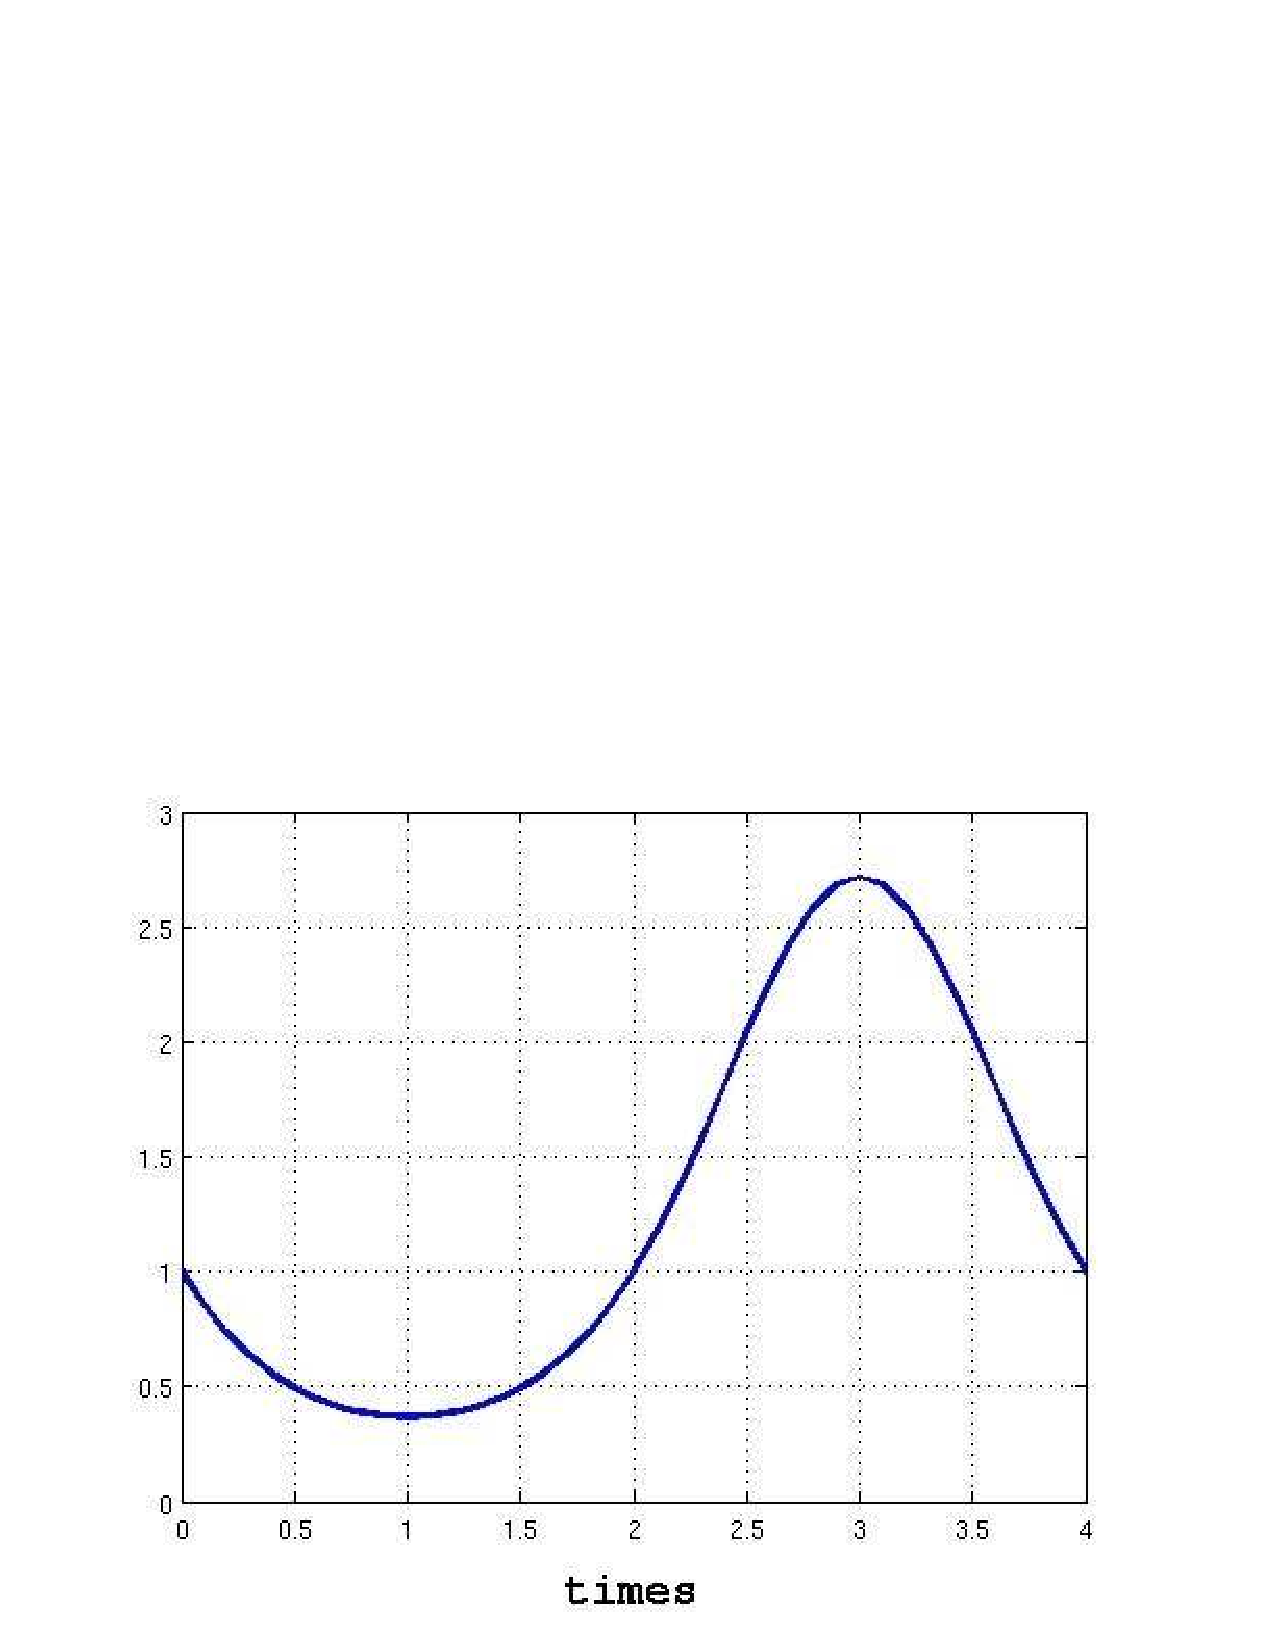
\includegraphics[width=6cm, height=8cm\textwidth]{figures/tempo.pdf}
\caption{The evolution of solution.} \label{temporal_solution}
\end{figure}
\end{center}
\begin{figure}[!h]
%\centering\includegraphics[width=12cm, height=12cm ]{figures/theta_bdf.eps}\\
%\centering
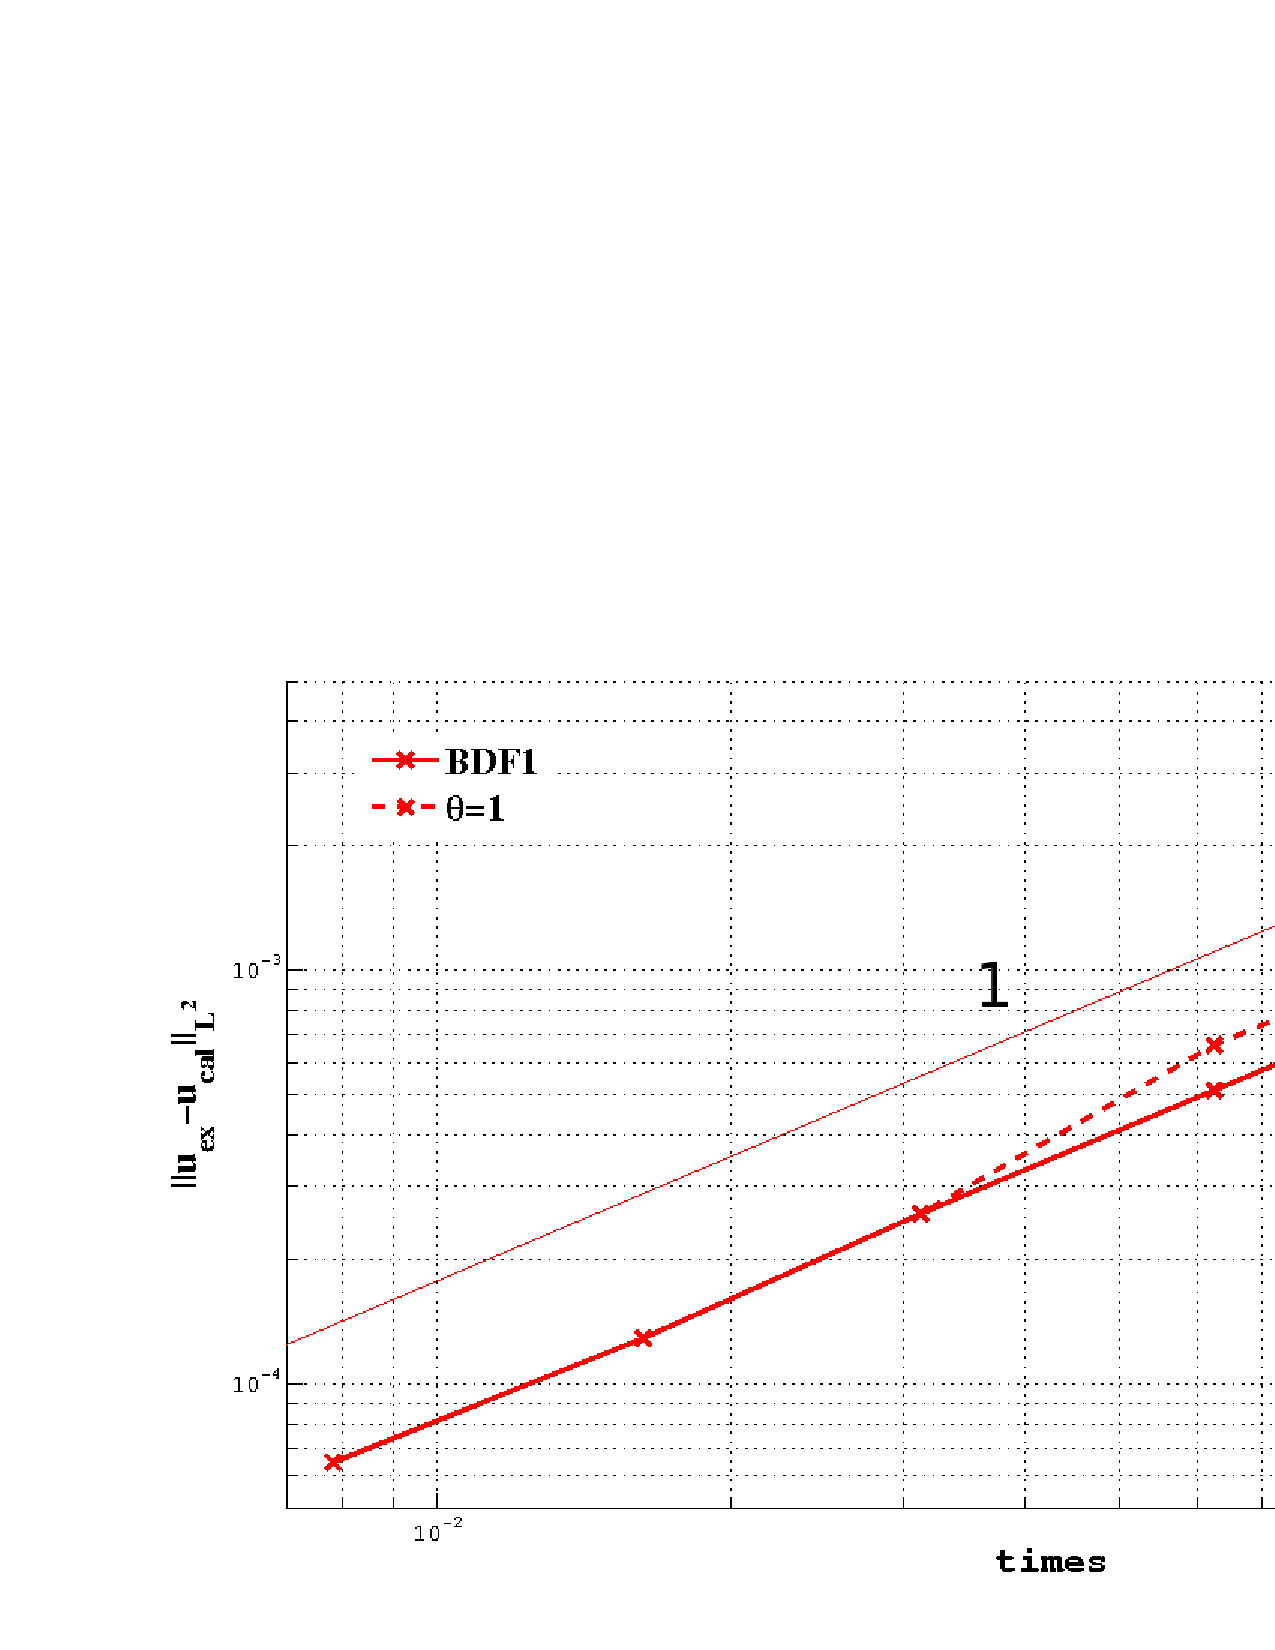
\includegraphics[width=6.25cm, height=8cm]{figures/P11_order1.pdf}
%\centering
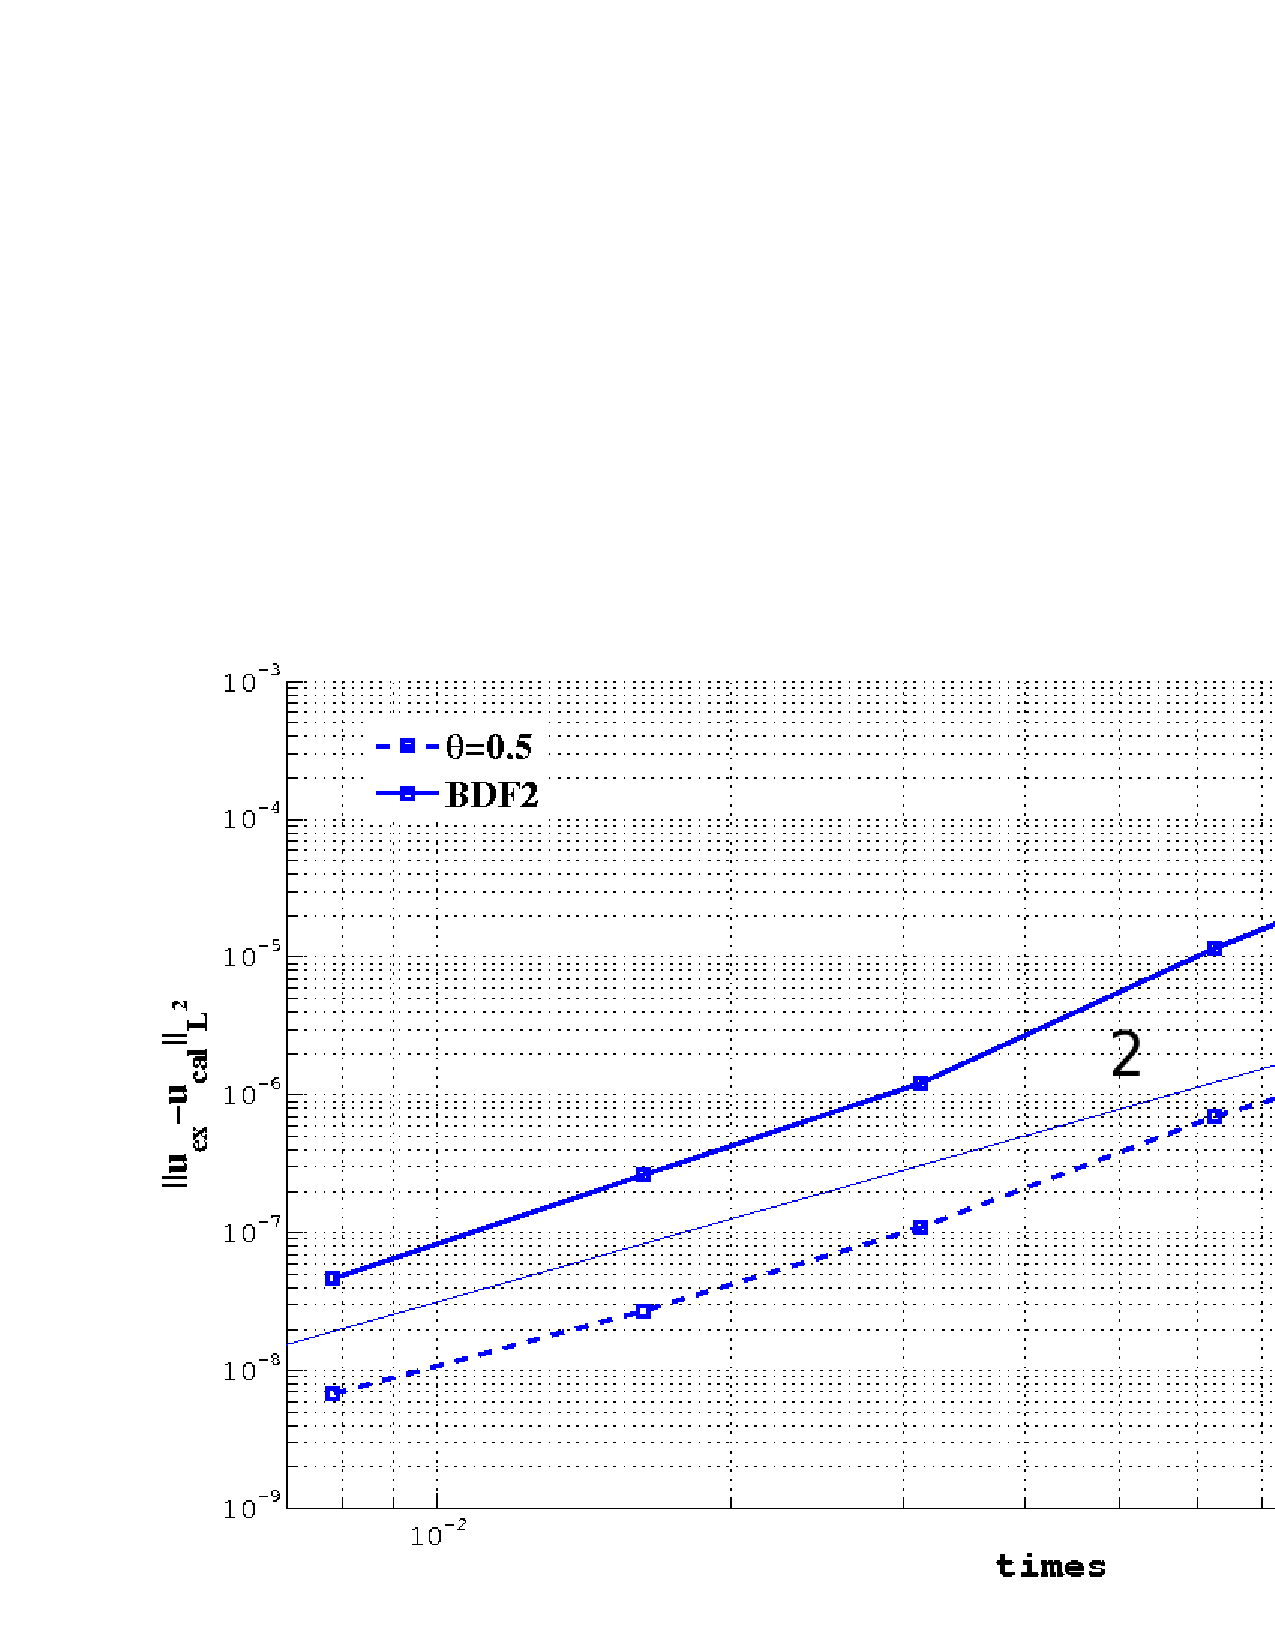
\includegraphics[width=6.25cm, height=8cm]{figures/P11_order2.pdf}\\
%\centering
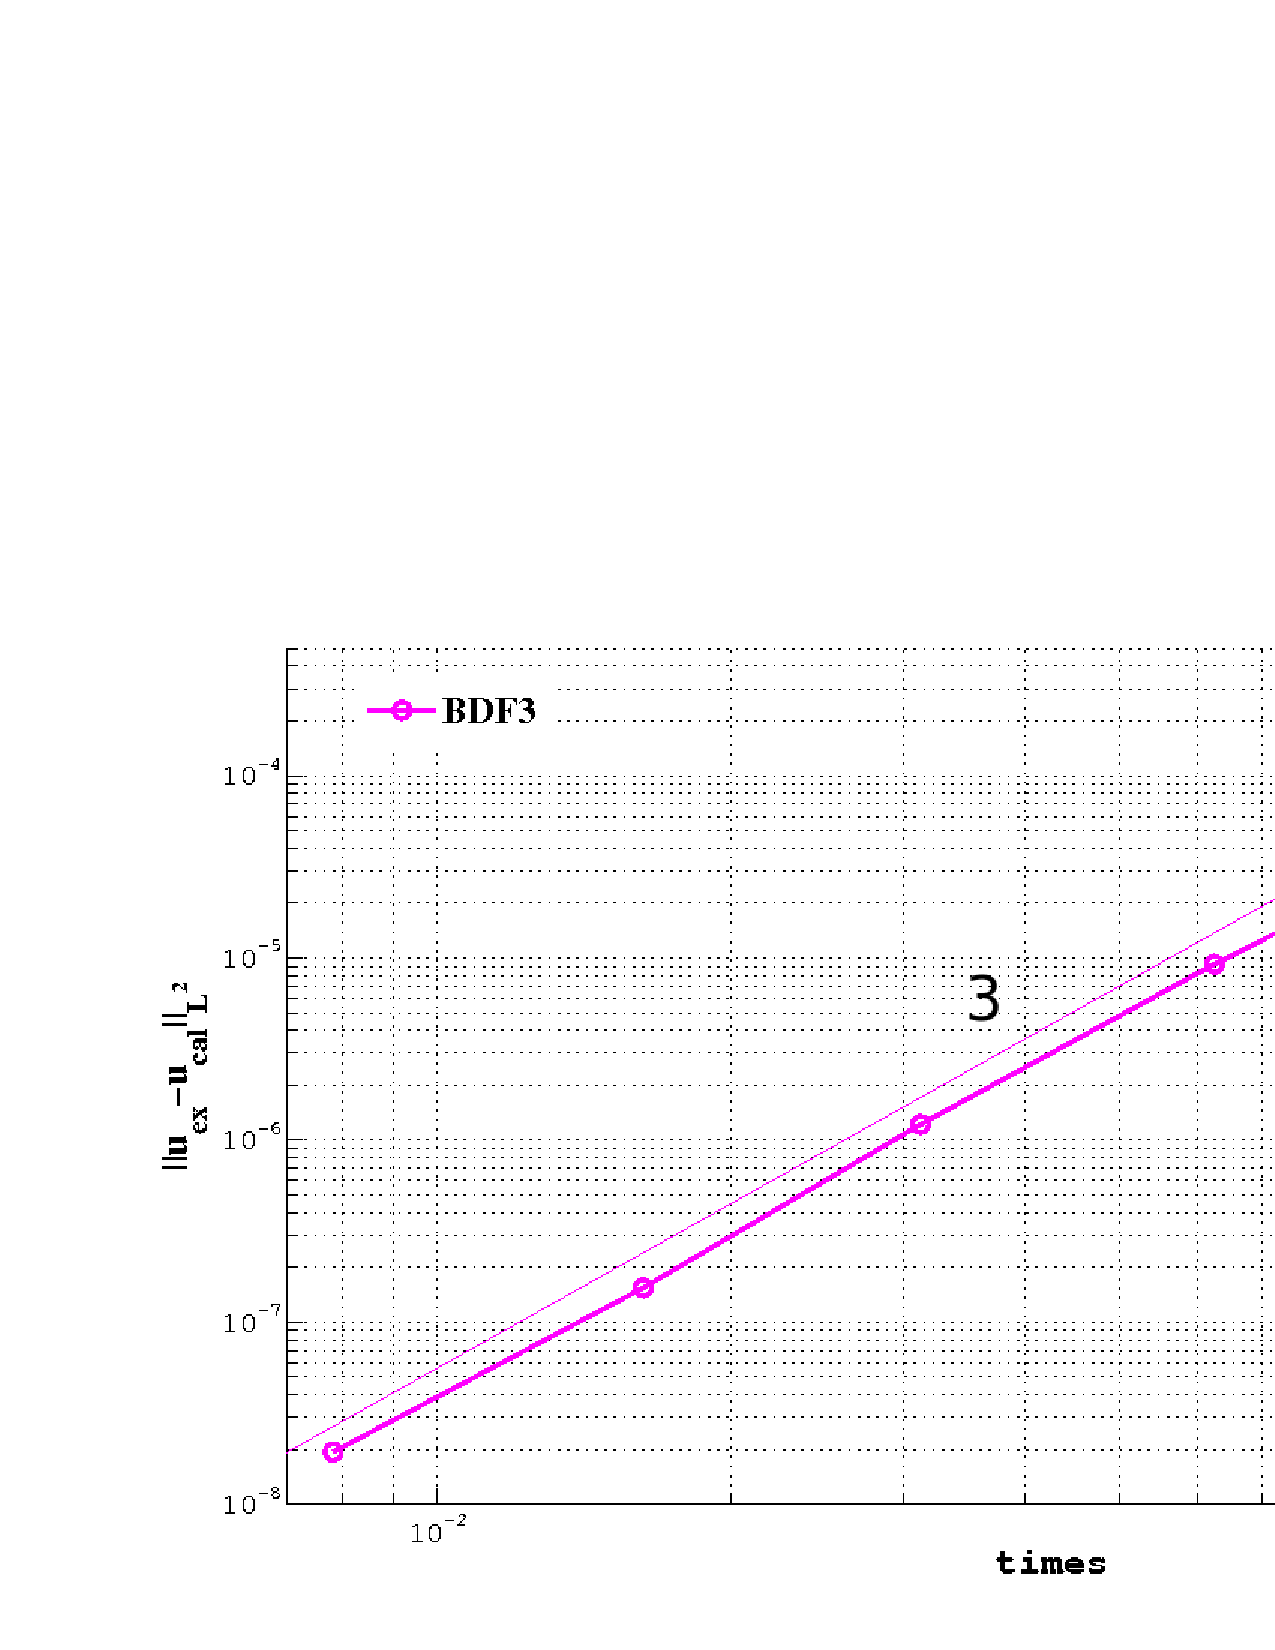
\includegraphics[width=6.25cm, height=8cm]{figures/P11_order3.pdf}
%\centering
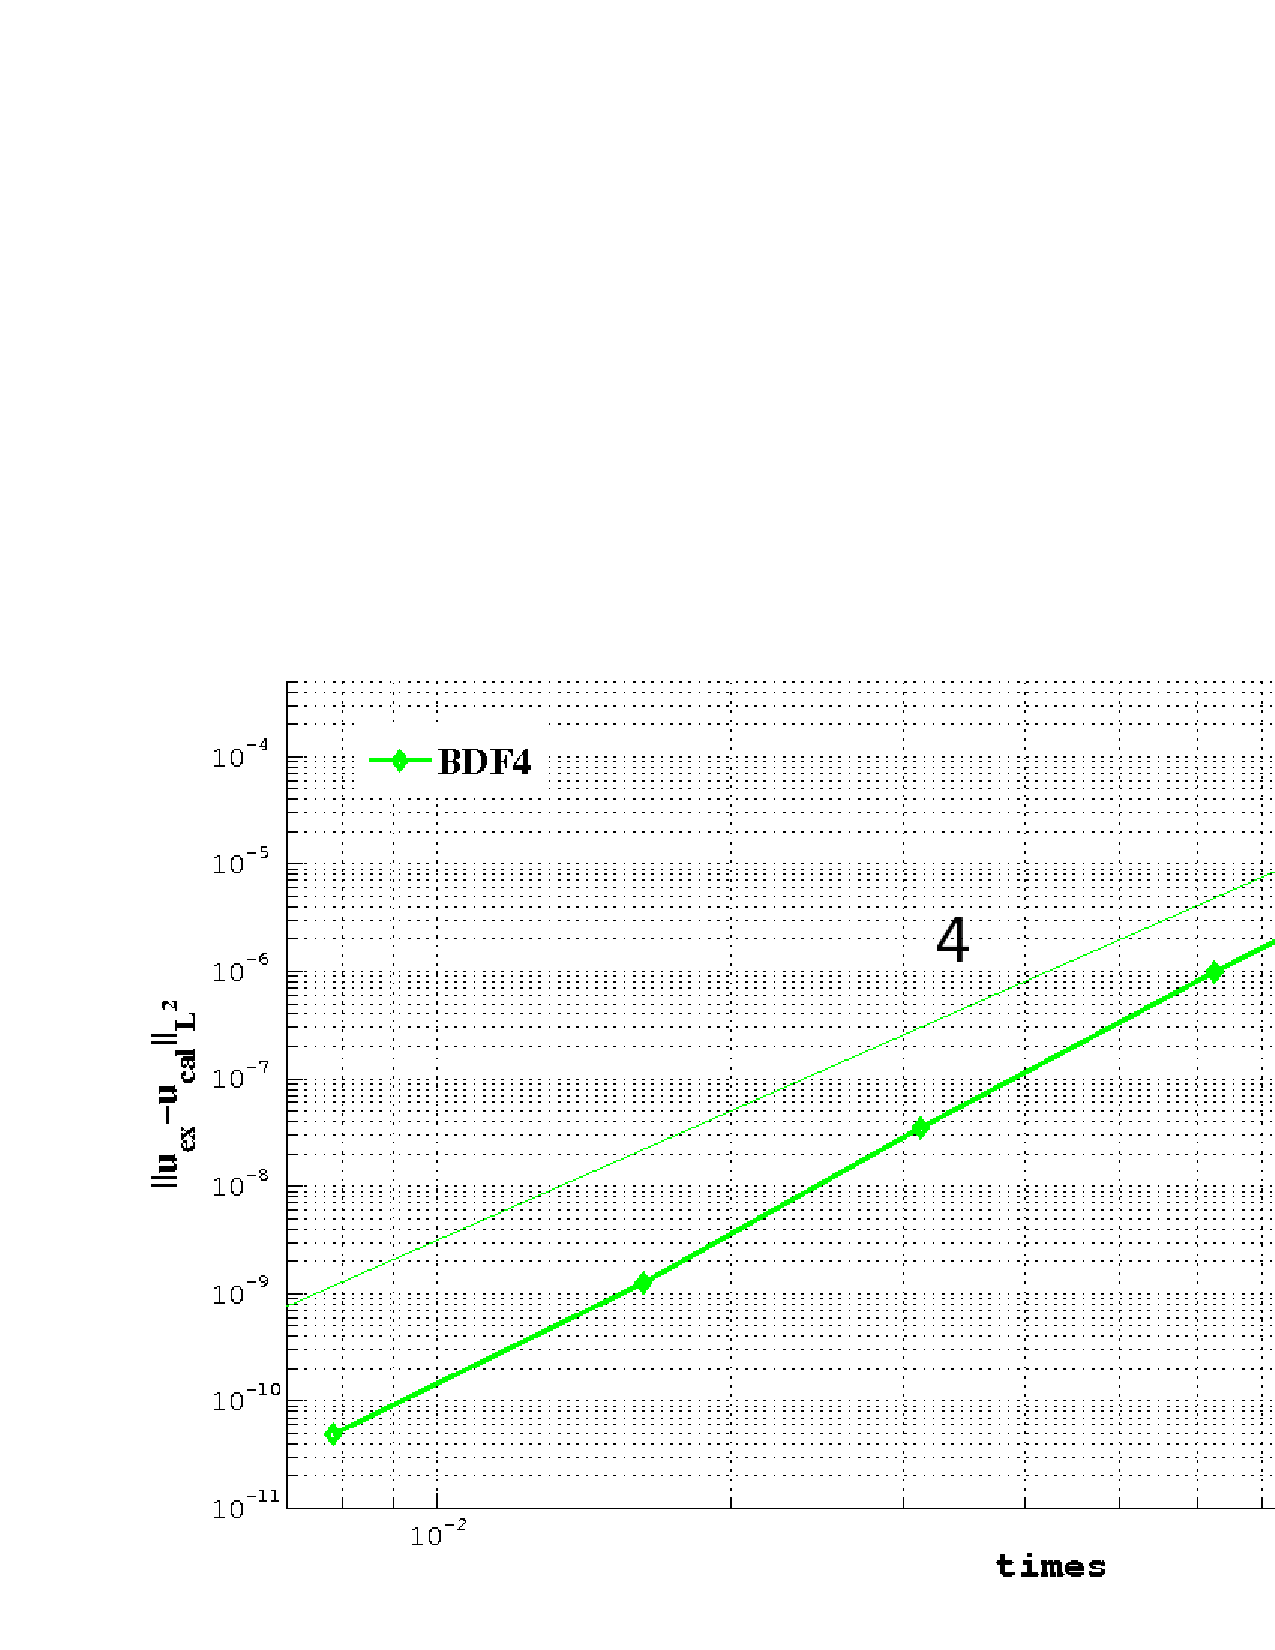
\includegraphics[width=6.25cm, height=8cm]{figures/P11_order4.pdf}
\caption{$L^2$ error of exact versus numerical solution computed with  BDF of order 1, 2, 3, 4 and $\theta$-method with
$\theta=1$ and $\theta=0.5$, respectively.}\label{acc1}
\end{figure}


\newpage
\clearpage
\subsubsection{test\_timeAdvance\_orderI}
In this section we present a possible implementation of time advance
scheme.\\
We consider the \verb"test_timeAdvance_orderI".\\
In file  \verb"data" we choose the parameters of time scheme:
\begin{verbatim}
[../time_discretitation]
//Newmark or theta-method
theta           = 0.5  #0.5

BDF_order       = 1  # 1, 2, 3, 4
\end{verbatim}
In the \verb"main" of the program we must choose the time advance scheme for
example:
\begin{verbatim}
  typedef boost::shared_ptr< TimeAdvance< vector_type > >   TimeAdvance_type;

 std::string TimeAdvanceMethod =  dataFile(
                                 "problem/time_discretization/method",
                                 "Newmark");

 TimeAdvance_type
 timeAdvance(TimeAdvanceFactory::instance().createObject(TimeAdvanceMethod));

  UInt OrderDev = 1;

if (TimeAdvanceMethod =="Newmark")
    timeAdvance->setup( dataProblem.getNewmark_parameters() , OrderDev);

  if (TimeAdvanceMethod =="BDF")
    timeAdvance->setup(dataProblem.getBDF_order() , OrderDev);
\end{verbatim}
where \verb"timeAdvanceMethod" is a
string and defines the temporal scheme read  from data
file; while \verb"timeAdvance" is an object coupled with a temporal scheme,
the builder  have two variables: the first define the parameters of
the temporal scheme and the second
defines the maximum order of the
time derivate (1 or 2).\\
Given that in this case we known the initial condition and the exact
solution,  we can initialize the vector \verb"_M_unknowns" as:
\begin{verbatim}

//evaluate disp and vel as interpolate the bcFunction d0 and v0

   std::vector<vector_type> uv0;

   if(TimeAdvanceMethod =="Newmark")
     {
    uv0.push_back(*U);
    uv0.push_back(*V);
     }
    if(TimeAdvanceMethod =="BDF")
      {
	for ( int previousPass=0; previousPass < dataProblem.getBDF_order() ;
              previousPass++)
	  {
	   Real previousTimeStep = -previousPass*dt;
	    FESpace.interpolate(uexact, *U, previousTimeStep );
	    uv0.push_back(*U);
	  }
      }
   timeAdvance->initialize_unk(uv0);
   timeAdvance-> setDeltaT(dataProblem.getTimeStep());
\end{verbatim}

In the solver we build the matrices of the  system and then we create a
temporal loop, where we update \verb"\fbf_V", the \verb"rhs" of the problem and
solve the problem, and update \verb"_M_unknowns".\\
In this part, the program is the same for both  Newmark and bdf schemes:
\begin{verbatim}
  double alpha = timeAdvance->coeff_der( 0 ) / ( dt );
  rhs *=0;
  rhsV = timeAdvance->time_der(dt);                 // update f_v
  FESpace.L2ScalarProduct(source_in, rhs, time);   //evaluate the rhs
  rhs += problem.matrMass() * rhsV;                // f + M f_v
  problem.updateSystem(alpha, rhs );               // update the system
  problem.iterate( bcH );                          // solve the system
  timeAdvance->shift_right(problem.u());         // update _M_unknowns
\end{verbatim}

We evaluate the $L^2$ and $H^1$ norms
of solution:
\begin{verbatim}
 AnalyticalSol uExact;
 Real H1_Error, H1_RelError, L2_Error, L2_RelError;
 L2_Error = FESpace.l2Error(uExact, uComputed, time ,&L2_RelError);
 H1_Error = FESpace.h1Error(uExact, uComputed, time ,&H1_RelError);
\end{verbatim}
where \verb"AnaliticalSol" is a
bcfunction in which is defined the
solution and the gradient of  the solution.\\

\subsection{Problem II}
We consider the following problem
\begin{equation}\label{ex2}
\left\{
\begin{array}{ll}
\displaystyle\frac{\partial^2 \ubf}{\partial t^2} -\Delta \ubf = \fbf & \text{in}\quad
\Omega\times [0,T],\\
\displaystyle\ubf(\xbf, 0) =  \ubf_0(\xbf)  & \text{in}\quad \Omega,\\
\displaystyle\frac{\partial^2 \ubf}{\partial t^2} =  \vbf_0(\xbf)  & \text{in}\quad \Omega,\\
\displaystyle\ubf(\xbf, t) = \psibf(\xbf, t)   & \text{on}\quad \partial\Omega\times[0,T],
\end{array}
\right.
\end{equation}
where $\Omega=[-0.5, 0.5]^3$ and $T=4$.
We choose $\fbf$, $\psibf$, $\ubf_0$ and $\vbf_0$, such that the exact solution
is given again by \eqref{u1ex1} and  evaluate the error
among the exact  and numeral solution in the $L^2$-norm  at
 time $t=3$, see Figure \ref{acc2}.
\begin{figure}[!h]
%\centering\includegraphics[width=12cm, height=12cm ]{figures/BDF2_order2.eps}\\
\centering
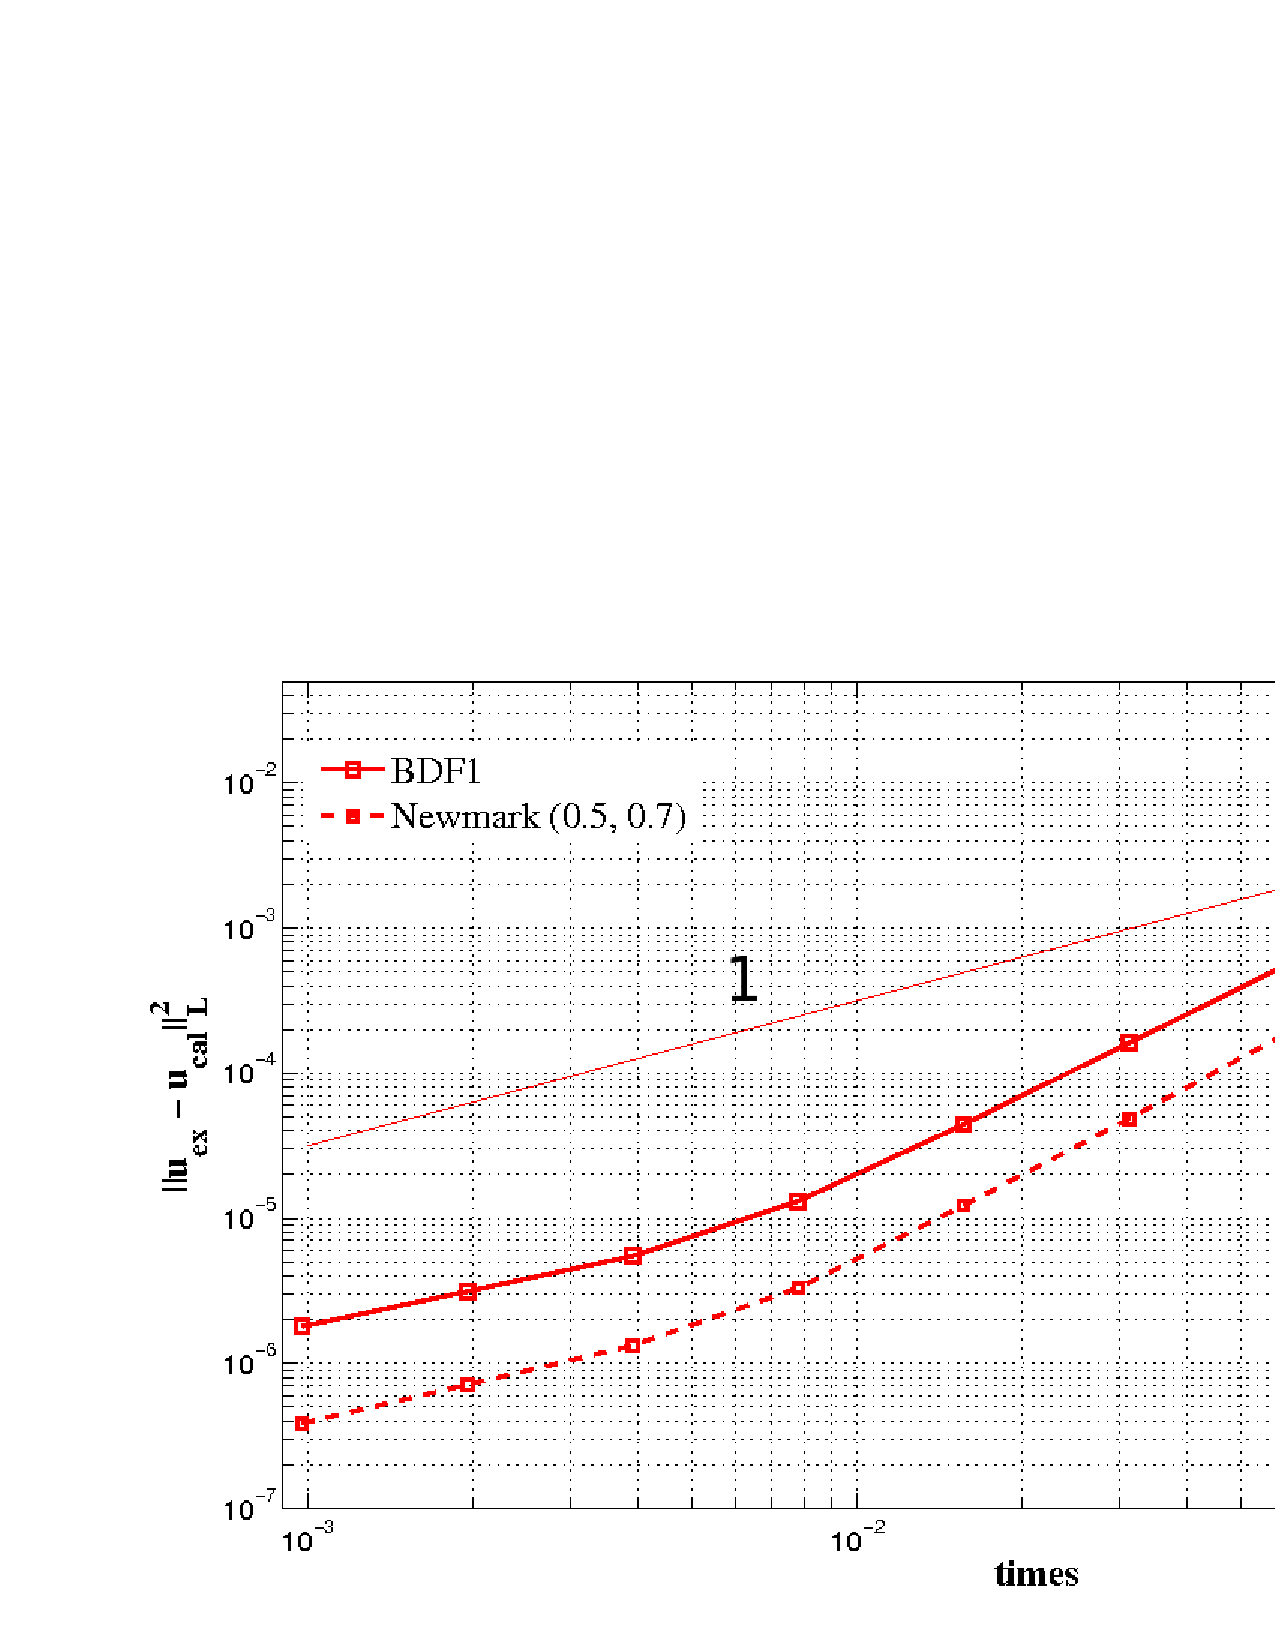
\includegraphics[width=8cm, height=10cm]{figures/P21_order1.pdf}
\centering
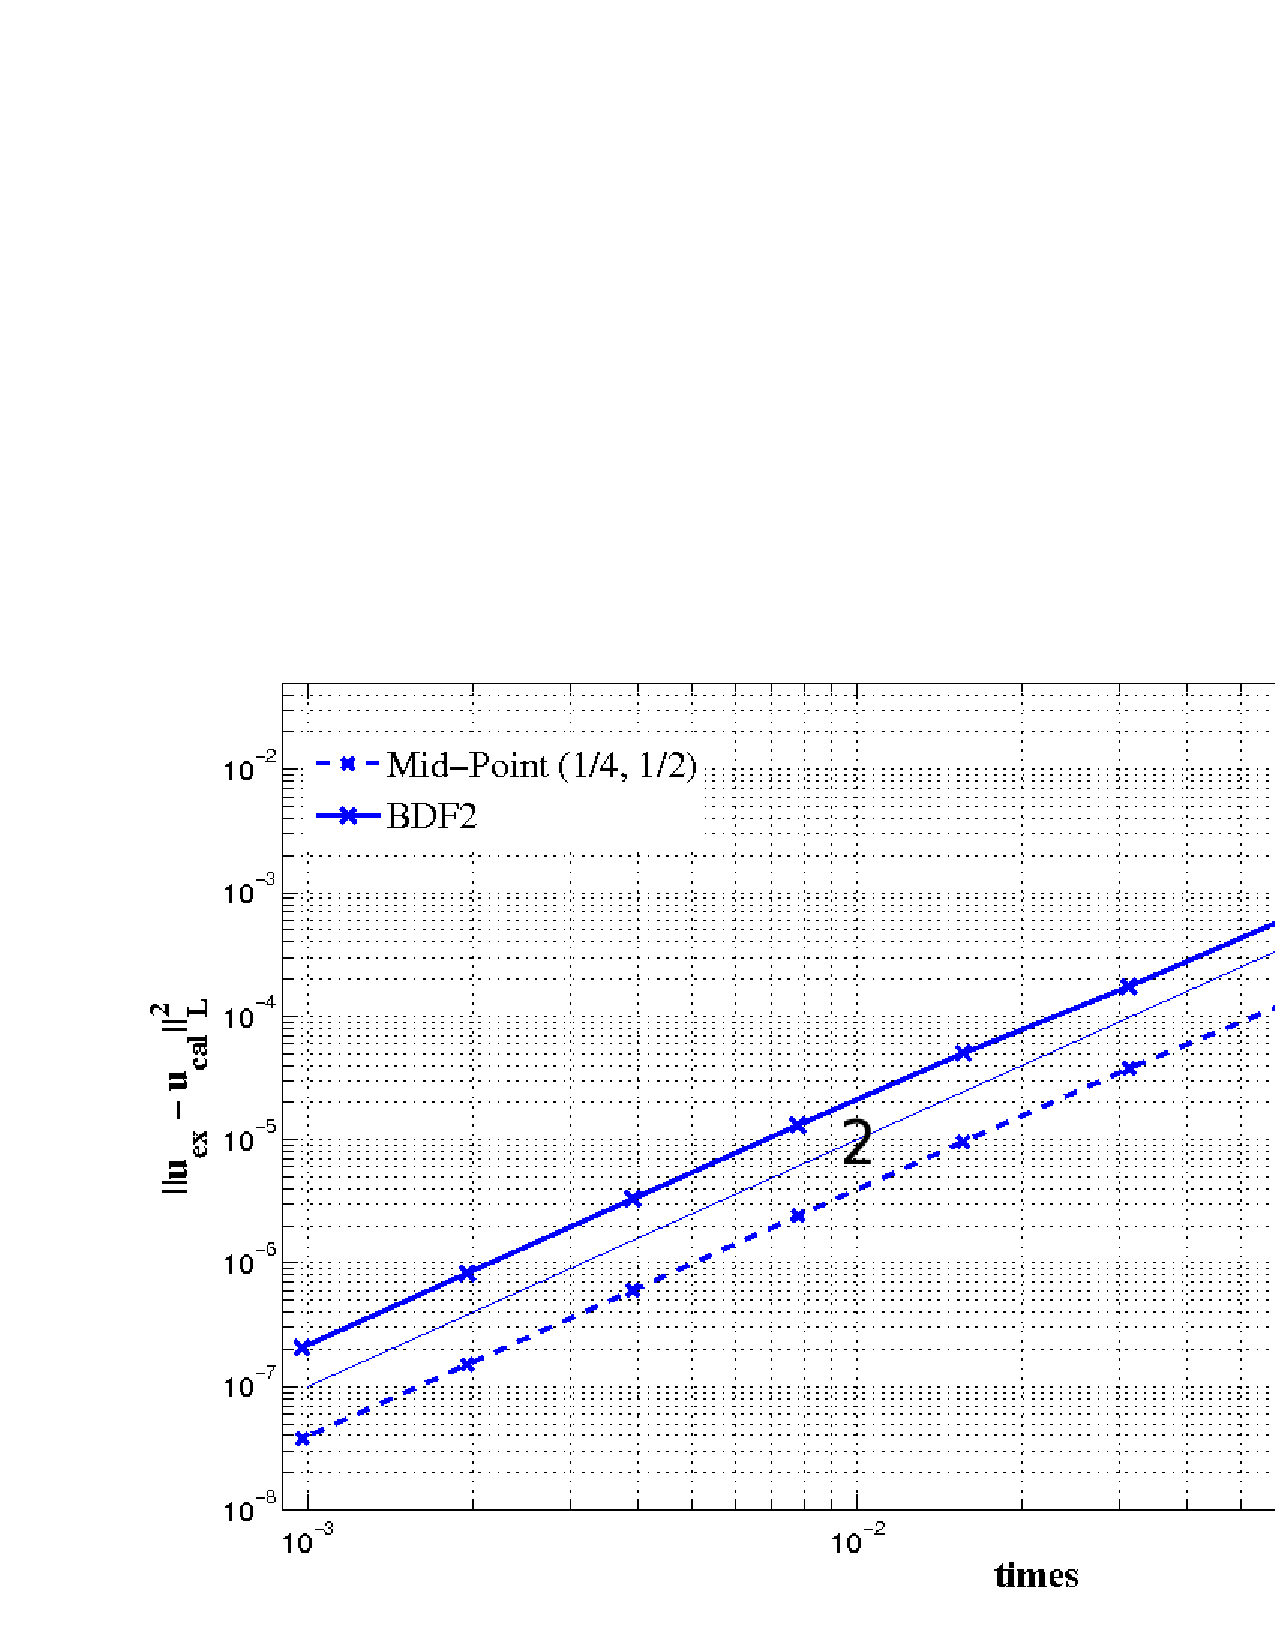
\includegraphics[width=8cm, height=10cm]{figures/P21_order2.pdf}
\end{figure}
\begin{figure}[!h]
\centering
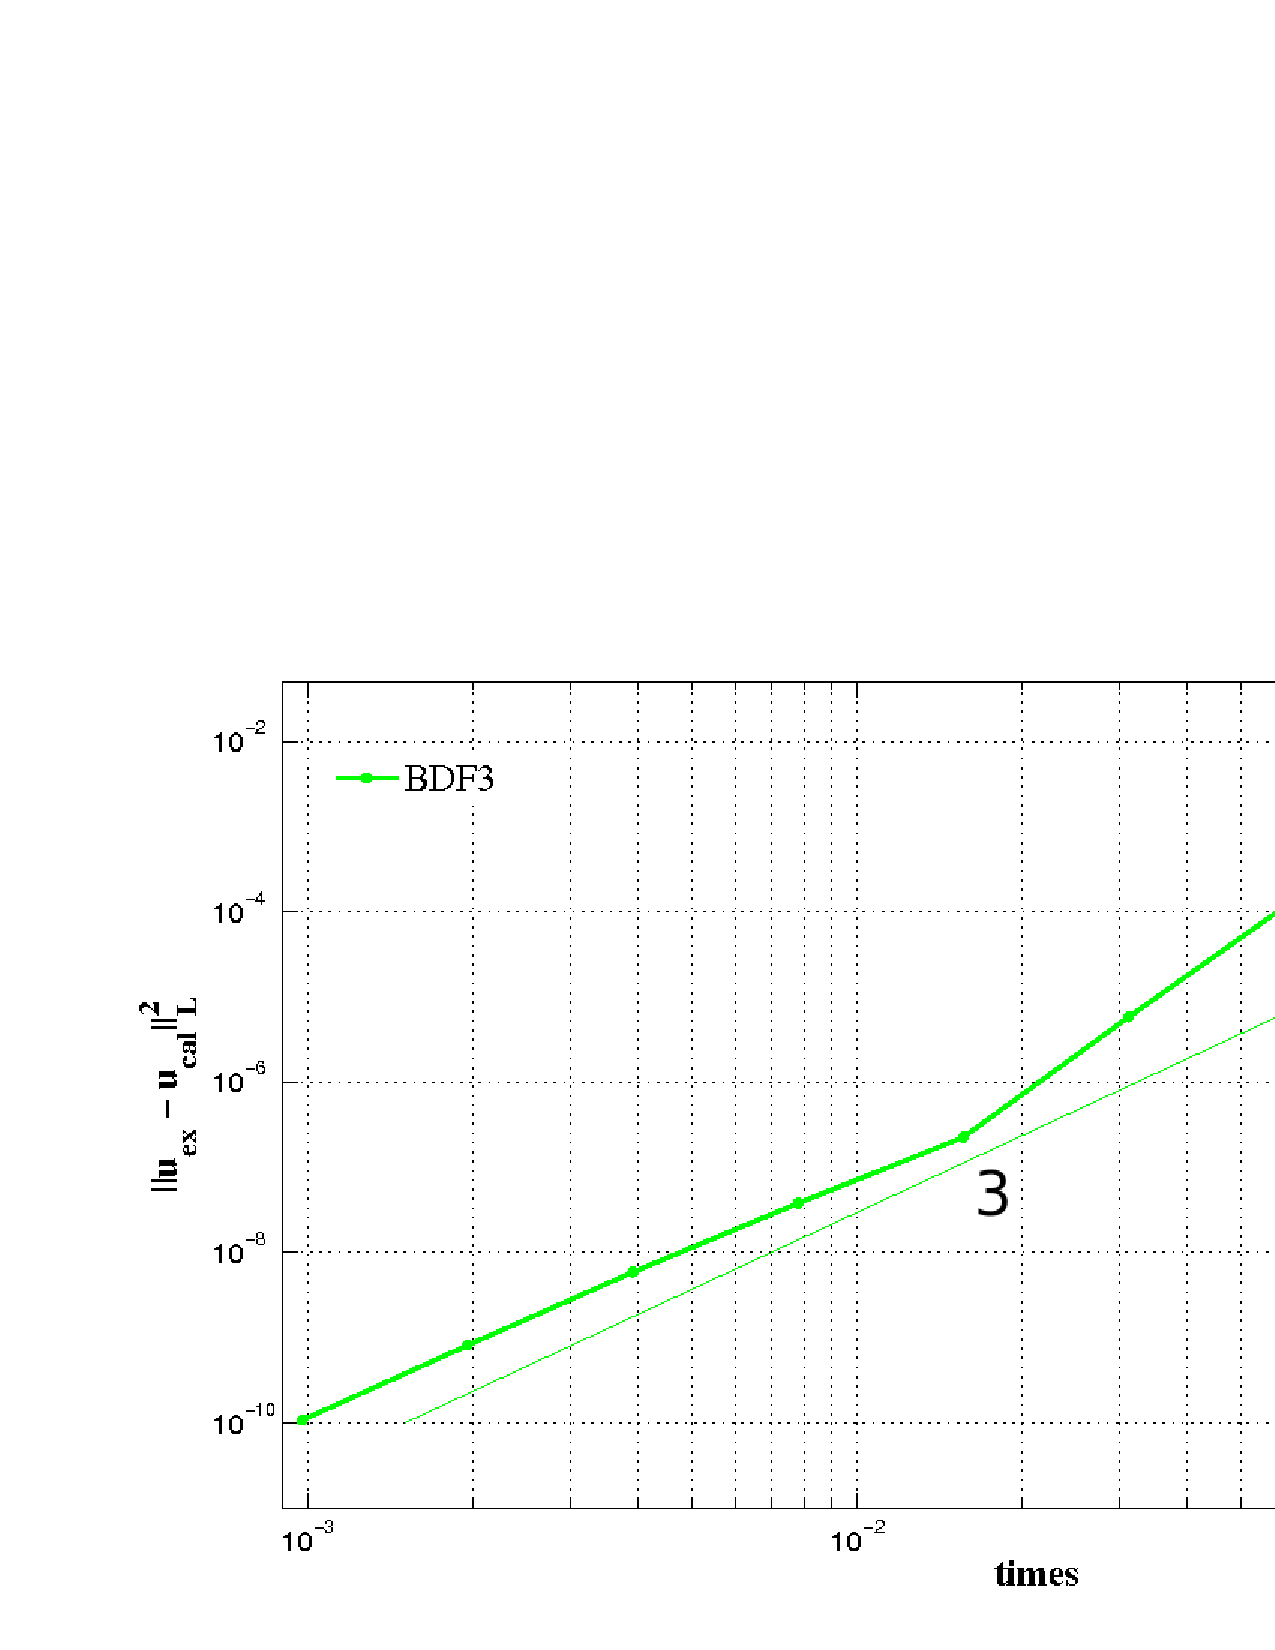
\includegraphics[width=6.5cm, height=9cm]{figures/P21_order3.pdf}
\caption{$L^2$ error of exact versus numerical solution computed with
  BDF of order 1, 2, 3, and Newmark with
$\theta=0.25$, $\gamma=0.5$ and $\theta=0.5$, $\gamma=0.7$, respectively.  }\label{acc2}
\end{figure}
\clearpage
\newpage
\subsubsection{test\_timeAdvance\_orderII}
The program is very similar to the previous example.
In file \verb"data" we introduce the parameters $(\theta, \gamma)$ of
Newmark scheme or the order $p$ of BDF.
\begin{verbatim}
[../time_discretitation]
//Newmark or theta-method
theta           = 0.25  # 0.5
gamma           = 0.5   # 0.7
BDF_order       = 1     # 1, 2, 3, 4
\end{verbatim}
In the main the variable \verb"orderdev" is $2$ and in the temporal
loop we have
\begin{verbatim}
  double xi = timeAdvance->coeff_derOrder2( 0 ) /( dt*dt);
  rhs *=0;
  rhsW = timeAdvance->time_der2(dt);                // update f_w
  FESpace.L2ScalarProduct(source_in, rhs, time);   //evaluate the rhs
  rhs += problem.matrMass() * rhsW;                // f + M f_w
  problem.updateSystem(xi, rhs );                  // update the system
  problem.iterate( bcH );                          // solve the system
  timeAdvance->shift_right(problem.u());            // update _M_unknowns
\end{verbatim}
 When we use Newmark we have also to call \verb"timeAdvance->time_der(dt)" because $\fbf_V^{n+1}$ always need when we call
 the function \verb"shift_right()".

% \subsection{Solid Problem:}
% We consider the linear elasticit model, given  by (\emph{Saint Venant-Kirchhoff}) equation
%  \begin{equation}\label{SVK}
% \displaystyle\rho_s\partial_{tt}\etabf-\nabla\cdot\textbf{T}_s=\textbf{f}_s
% \qquad\text{in} \quad(0,T) \times\Omega^0_s
%  \end{equation}
% where $\textbf{T}_s$ is a Cauchy tensor.\\
% An analitical solution of \eqref{SVK} is:
% $$ \etabf =
%  \begin{bmatrix}
%    X_1(\cos\theta-1) -X_2\sin\theta \\
%    X_1\sin\theta+X_2 (\cos\theta-1) \\
%    0
%  \end{bmatrix},
% $$
% and the force term is:
% $$
% \fbf_s=\begin{bmatrix}
%  -\rho_s\left( \ddot{\theta}  \big( X_1\sin\theta+ X_2\cos\theta
%    \big)+\dot{\theta}^2\big( X_1cos\theta -
%    X_2\sin\theta\big)\right)
% \\
% \rho_s\left( \ddot{\theta} \big(X_1\cos{\theta}-X_2\sin\theta \big) -
%   \dot{\theta}^2 \big(
%   X_1\sin{\theta}+X_2\cos\theta\big)\right)
% \\
% 0
% \end{bmatrix}
% $$


\section{Initial condition}\label{start}
In general we know only $\Ubf_0$ for first order problems and
$(\Ubf_0, \Wbf_0)$ for second order problems.
For $\theta$-method and Newmark we have to recostruct missing information
to build {\sl state} vector \verb"_M_unknowns":
\begin{itemize}
\item the first order problem  given by \eqref{order1}.
\begin{equation}\label{Vbf00}
M \Wbf^0= \Fbf^0\quad\text{where}\quad \Fbf^0= \fbf^0 - A \Ubf^0
\end{equation}
\item[]We show a possible implementation. In the main we build right
  hand side and evaluate the solution $\Wbf_0$ with the function
  \verb"solve0" of the solver.
\begin{verbatim}
  vector_type v0(problem.U().getMap(), Repeated ); //v0 is Zero EpetraVector;
  FESpace.L2ScalarProduct(source_in, rhs0, 0);
  rhs0 -= *problem.getStiff()*u0;
  rhs0.GlobalAssemble();
  problem.solver0(v0, bch, rhs0);  //evaluate v0;
\end{verbatim}
 \item the second order problem given by \eqref{order2}:
\begin{equation}\label{Wbf00}
M\Abf_0= \Fbf^0, \quad\text{where}\quad \Fbf^0= \fbf^0- D\Wbf_0-A \Ubf_0.
\end{equation}
\item[]We show an possible implementation. In the main we build right
  hand side and evaluate the solution $\Abf_0$ with the function
  \verb"solve0" of the solver.
\begin{verbatim}
  vector_type a0(problem.U().getMap(), Repeated ); //a0 is  Zero EpetraVector;
  FESpace.L2ScalarProduct(source_in, rhs0, 0);
  rhs0 -= *problem.getStiff() * u0;
  rhs0 -= *problem.getDamping() *v0;
  rhs0.GlobalAssemble();
  problem.solver0(a0, bch, rhs0);  //evaluate a0
\end{verbatim}
The function \verb"solver0" solve the problem \eqref{Vbf00} and
\eqref{Wbf00}.
\begin{verbatim}
template <typename Mesh, typename SolverType>
void SecondOrderSolver<Mesh, SolverType>::
solver0( vector_type& sol0,  bchandler_raw_type& bch, vector_type  rhs0 )
{
  vector_type rhsFull(rhs0);
  applyBoundaryConditions( *matrFull, rhsFull, bch);
  prec_type prec;
  std::string precType ="Ifpack" ;
  prec.reset( PRECFactory::instance().createObject( precType ) );
  prec->buildPreconditioner(M_mass);
  Real condest = prec->Condest();
  M_linearSolver->setPreconditioner(prec);
  M_linearSolver->setMatrix(*M_mass);
  int numIter =  M_linearSolver->solve(sol0, rhs0);
}
\end{verbatim}
\end{itemize}

\end{document}



